
In this section we show a motivating example and formally introduce our approach: {\em \textbf{D}iversity \textbf{M}aximization \textbf{S}peedup} (\textsc{Dms}). \textsc{Dms} employs trend analysis to give priorities to test cases that can quickly increase the diversity of suspiciousness scores generated by fault localization techniques for various program elements.
%It employs trend analysis to speedup the diversification process by identifying promising program elements that are likely to increase diversity as more test cases that execute them are selected.
In the subsections, we illustrate its intuition and formally define it as a variant of test case prioritization.
%show a motivating example and describe the details of our approach.

\subsection{Running Example Revisited}\label{sec.motive}



\begin{figure}[!htbp]
    \centering
%    \vspace{-0.9cm}
    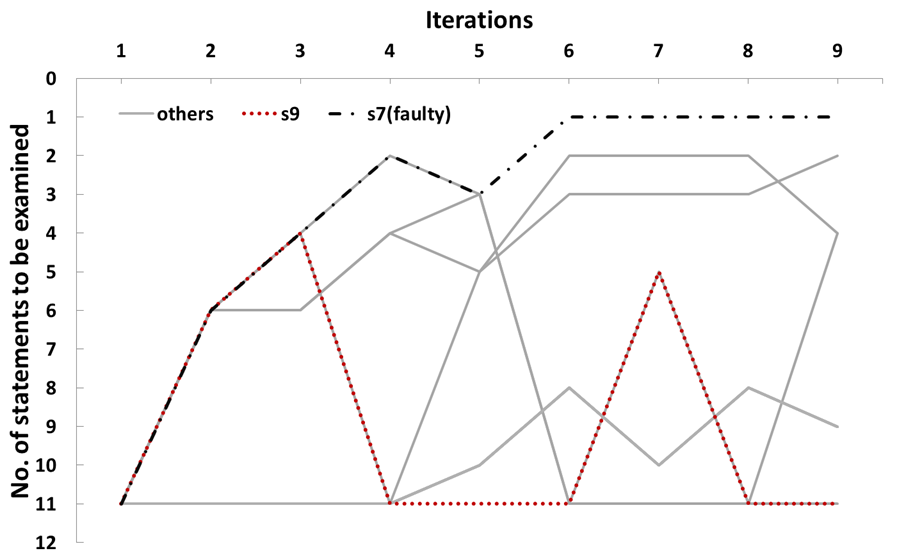
\includegraphics[width=12cm]{motive_1.png}
   % \vspace{-0.8cm}
    \caption{Motivating Example}
    \label{fig:motive_1}
\end{figure}

We use the running example (Figure~\ref{motiv_example}) to explain the intuitions for
\textsc{Dms}. With sufficient test cases, an effective fault localization technique is more likely to assign high suspiciousness scores to faulty program elements while assigning low scores to non-faulty elements, and each element should be assigned a unique rank according to their suspiciousness scores to facilitate further investigation (such as the scores shown in the last three columns in Figure~\ref{motiv_example}).

With fewer test cases, a fault localization technique may not be able to achieve an effective ranking. Figure \ref{fig:motive_1} shows the evolution trend of the ranks of the running example's program statements based on their {\em Ochiai}~\citep{Abreu:2009.jss} scores as test cases are added one by one. The test cases are added by \textsc{Raptor} which is the existing best approach in the literature~\citep{Alberto2011} for selecting test cases for fault localization. In this figure, the horizontal axis represents the number of iterations to select test cases. In each iteration, one test case is picked from the unlabeled test case pool $T_\mathcal{U}$.
The vertical axis is the rank\footnote{\scriptsize Program elements with the same suspiciousness score are assigned the same {\em low} rank since developers are expected to investigate all of the elements having the same score if they are ever going to investigate one. For example, if statements $s_{1}$, $s_{2}$, $s_{3}$ have the highest suspiciousness score, then the ranks of the 3 statements are all 3.}
of a statement sorted based on suspiciousness. Each line in the figure depicts the evolution of the suspiciousness rank for one specific statement. For example, $s_{7}$ (the faulty statement) is ranked $11^{th}$ in the first iteration, and $6^{th}$ in the second iteration.

This figure shows that the ranks of different statements may evolve in different ways as more test cases are added. Specifically, some statements keep rising in general (e.g., $s_{7}$); some others oscillate back and forth (e.g., $s_{9}$).
Ideally, we should only use test cases that could enable a fault localization technique to assign elements the scores close to the final score when all test cases are used.
Comparing to the changes of $s_{7}$, the oscillation of $s_{9}$ is less important as its final rank is the same as its initial rank.
Thus, when we add test cases, we should look for test cases that could offer more {\em changing opportunities} to ``promising'' elements like $s_{7}$ (with clear trend) instead of $s_{9}$ so that the ranks (for both $s_{7}$ and $s_{9}$) may quickly approach their final position.

\begin{comment}
Observing Figure \ref{fig:motive_1} we can see the ranks of different statements evolve in different ways as more test cases are added. The ranks of some statements decreases gradually (e.g., $s_{7}$'s rank), while the ranks of some elements oscillates back and forth (e.g., $s_{9}$'s rank). Elements whose ranks change much are interesting as they correspond to the increase in the diversity as more test cases are added.

\end{comment}

The following questions prompted us to define {\sc Dms}:

%\vspace{-4pt}
\begin{enumerate}
\item Can we analyze the change trend of every program element and identify ``promising'' elements with {\em high change-potentials} (i.e., elements whose ranks are likely to change much in a stable way)?
%\vspace{-2pt}
\item For program elements having high change-potentials, can we select appropriate test cases to speed up their rank changing process so that these elements can reach their final ranks faster (i.e., with fewer test cases)?
\end{enumerate}

%\vspace{-6pt}
\subsection{Formal Definition of DMS}

%\vspace{-6pt}
\begin{definition}[{\bf Diversity Maximization Speedup}]
Given (1) $T$, a set of test cases, (2) $PT$, the set of permutations of $T$, and (3) $k$, a positive integer, we use $p^k$ to represent a permutation $p\in PT$ truncated at length $k$, and $PT^k$ to represent all such truncated permutations (i.e., $PT^k=\{p^k|p\in PT\}$).

Then, with $f$, a function mapping $PT^k$ to real numbers, the problem of DMS is to find a permutation $p \in PT$ such that:
%\begin{center}
	$\forall{p_i^{k} \in PT^{k}}.$	$f(p^{k}) \geq f(p_i^{k})$, for the given $k$.
%\end{center}
\label{defn:diagnosticpriori}
\end{definition}

In Definition~\ref{defn:diagnosticpriori}, $f$ is an award function indicating the value of an ordering in $PT^{k}$, which in our case, would be the effectiveness of a fault localization technique based on $k$ labeled test cases.
%, which is a set of test cases of size $k$. Without the loss of generality, the definition assumes
%that higher award values are preferable to lower ones.
The number $k$ can be used as a labeling budget, indicating the number of test cases developers are willing to label for fault localization.
%Fault localization techniques would analyze traces corresponding to the execution of these test cases and rank program elements based on suspiciousness. Developers can then browse this list and inspect program elements one-by-one based on their suspiciousness. Thus, the goal is to minimize developer's cost in browsing the list of program elements to find the location of the bug. Specifically, given two ordered sets of test cases $p$ and $p'$, if by analyzing $p$, the fault localization tool can put the buggy program element higher in the suspiciousness list than the corresponding list produced by analyzing $p'$, then $f(p) \geq f(p')$.
Thus, the goal for {\sc Dms} is to quickly maximize the effectiveness of fault localization techniques with at most $k$ labeled test cases.
